% !TEX root = ../main.tex

\chapter{数值模拟和验证}\label{chap:4}

\section{数值模拟的模型设置}

为了从数值上说明随机化实验复杂设计的结果,我们采取以下\textbf{线性可加模型}模拟出实验结果$\mathbf{Y}$:
    \begin{equation}\label{linear Model}
        \textit{\textbf{Linear Model}}:\quad y_i (w_i) | \mathbf{x}_i = \beta_0 + \beta_1^{\top}\mathbf{x}_i+\tau w_i + \epsilon_i,
    \end{equation}
    其中$\epsilon_i \sim N(0,\ \sigma^2)$。

\begin{figure}[!htbp]
    \centering
    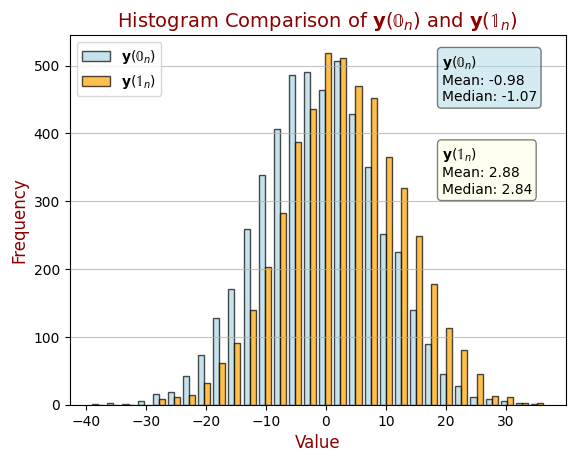
\includegraphics[width=0.75\linewidth]{figures/distributionOfy.png}
    \caption{$\mathbf{y}(\mathbb{0}_n)$和$\mathbf{y}(\mathbb{1}_n)$的频数直方图}
    \label{fig:distributionOfy}
\end{figure}

线性可加模型的参数$\beta_0$、$\beta_1$由均一分布随机抽取后标准化得到,而协变量$\mathbf{X}$从均值为$\mu_d$,方差为$\eta I_d$的多元正态分布中抽取。实验结果$y_i(0)=\beta_0 + \beta_1^{\top}\mathbf{x}_i+ \epsilon_i$和$y_i(1)=\beta_0 + \beta_1^{\top}\mathbf{x}_i+\tau + \epsilon_i$的频数直方图如\ref{fig:distributionOfy}所示。在图\ref{fig:distributionOfy}中,具体的参数设置为$n=5000, d=5, \tau=3, \mu_d = 0, \eta=1, \sigma^2=0.25$。图像中蓝色部分和黄色部分分别为将所有样本分配到对照组和实验组的结果:对于被分到对照组($w_i=0$)的样本$\mathbf{x}_i$,我们用蓝色标出;对于对于被分到实验组($w_i=1$)的样本$\mathbf{x}_i$,则选用黄色标出。在后续的随机化分组中,我们会选用固定的随机化出的协变量$\mathbf{X}$, 且为了形成有效的对照,所有随机化实验方案都使用相同的协变量$\mathbf{X}$。


\section{随机化方法与参数设置}
    我们将着重对重随机化、A/A 测试,区组随机化和分层随机化在代码上进行实现,并根据分组结果计算$\hat\tau$。为了避免偶然性,每种随机化方法都会重复10000次,并展示相应方法计算出的$\hat\tau$在均值和方差上的结果。具体每种随机化方法的设计如下。
    
\subsection{重随机化}
\begin{figure}[!htbp]
    \centering
    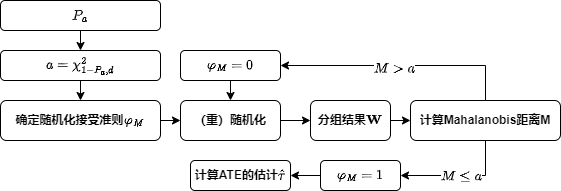
\includegraphics[width=0.8\linewidth]{figures/Rerandomization.drawio.png}
    \caption{重随机化实验设计的具体流程}
    \label{fig:RerandomizationDesign}
\end{figure}
此处我们采用可接受准则为$\varphi_M$的重随机化,为了平衡好计算时间与受试者在组间的分布差异,我们选取了$P_a=0.5$,进而可以求得相应的Mahalanobis距离的阈值$a=4.35$。具体实验设计流程如图\ref{fig:RerandomizationDesign}所示,理论上我们期望观察到重随机化后的$\hat{\tau}$在均值上应当和组间样本量相等的完全随机分组相近,但在方差上有所下降。

\begin{figure}[!htbp]
    \centering
    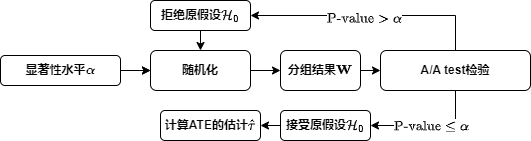
\includegraphics[width=0.8\linewidth]{figures/Chapter4AAtest.drawio.png}
    \caption{A/A test 实验设计的具体流程}
    \label{fig:AAtestDesign}
\end{figure}

\subsection{A/A 测试}

A/A 测试 的流程如图\ref{fig:AAtestDesign},和\ref{chap3:AAtest}中的阐述保持了一致。此处我们需要提前设置显著性水平$\alpha=0.05$, 也即是我们容许的组间存在显著差异的可能性为5\%。当分组结果$\mathbf{W}$没有通过A/A测试时,我们将拒绝此次分组结果并重新分组,直至出现通过A/A 测试的分组。

\subsection{区组随机化}
\begin{figure}[!htbp]
    \centering
    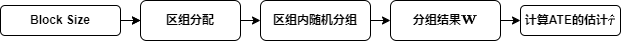
\includegraphics[width=0.8\linewidth]{figures/Chapter4Block.drawio.png}
    \caption{区组随机化实验设计的具体流程}
    \label{fig:BlockDesign}
\end{figure}

在进行如图\ref{fig:BlockDesign}的区组随机化之前我们需要设置每个区组的大小(Block Size),此处我们选取$\text{Block Size} = 2$,也即每个区组内部会有两名受试者分别被分到实验组和对照组。在医学实验中,受试者往往是逐一进入每个区组直至区组满员而进入下一个区组。但是我们预先生成了所有协变量$\mathbf{x}$,而每个样本之间没有先后次序之分,因此我们采取先将受试者随机分配至$n/2$个区组中,再在区组内进行二次随机分配的方案。可以预见的,此处的区组随机化后的分组结果并不会优于组间样本量相等的完全随机分组,这是由于我们并没有引入顺序影响的误差。


\subsection{分层随机化}
\begin{figure}[!htbp]
    \centering
    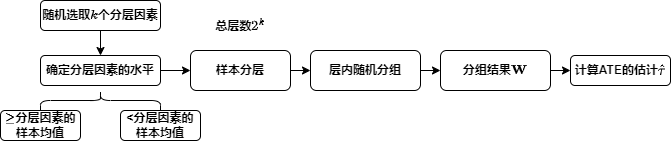
\includegraphics[width=0.8\linewidth]{figures/Chapter4Stratified.drawio.png}
    \caption{分层随机化实验设计的具体流程}
    \label{fig:StratifiedDesign}
\end{figure}

在进行分层随机化前,实验设计者需要确定对实验结果影响较大的混杂因素如性别、年龄等。在此处由于所有协变量$\mathbf{X}$由从正态分布中随机生成,因而不存在上述明确可以选择的分层因素。为此,我们采取随机选取$k=3$($k<d$)个维度作为分层因素,分层因素的水平人为设置为大于等于分层因素的样本均值和小于分层因素的样本均值。因而我们可以得到$2^k$个层。在此基础上,我们根据图\ref{fig:StratifiedDesign}中的流程,在样本的分层之后,在每个层次内部随机分组,进而得到最终的分组结果$\mathbf{W}$。

\section{随机化方法对$\hat{\tau}$的影响}
根据使用不同的随机化设计重复10000次实验分组之后,我们可以计算出5组$\hat{\tau}$。图\ref{fig:Comparative Boxplot Analysis}分别展示这5组$\hat{\tau}$的箱线图结果,红色虚线则标注出了真实的$\tau$的值。图\ref{tab:Comparative stats Analysis of Average Treatment Effects}则直接展示了5组平均处理效应的估计$\hat{\tau}$的均值和方差的结果。
\begin{figure}[!htbp]
    \centering
    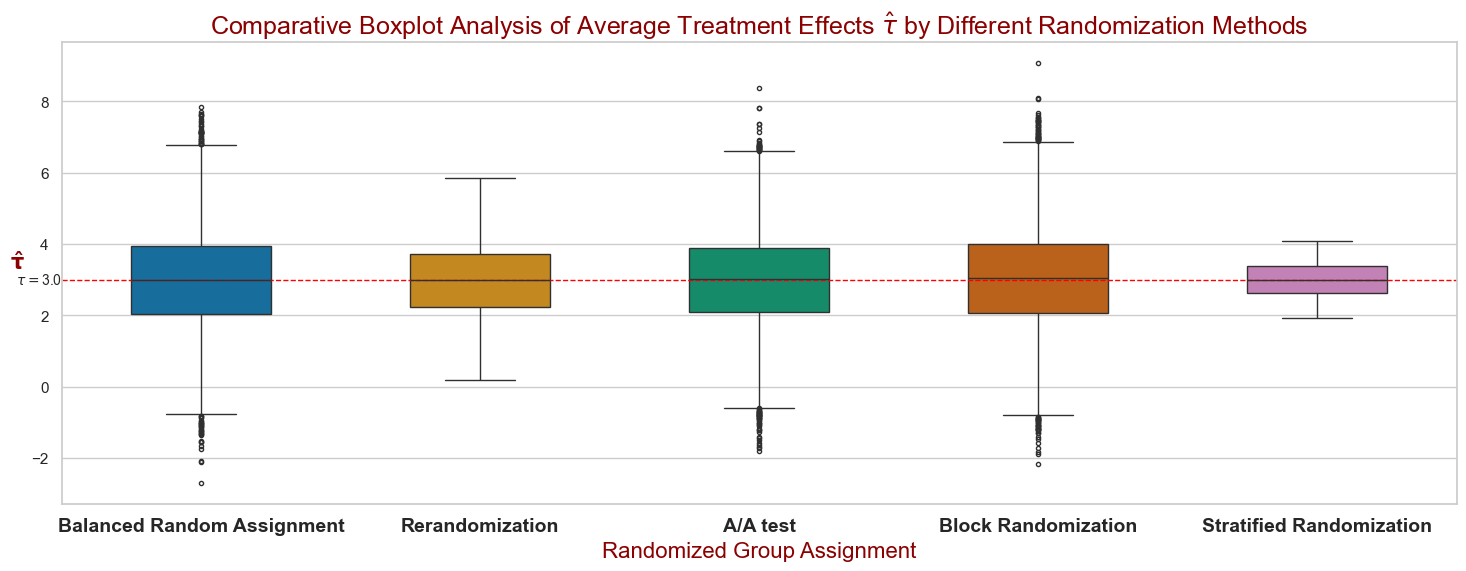
\includegraphics[width=1.00\linewidth]{figures/Comparative Boxplot Analysis of Average Treatment Effects.png}
    \caption{不同随机化方法下平均处理效应$\hat{\tau}$的比较性箱线图分析($\tau=3.0$)}
    \label{fig:Comparative Boxplot Analysis}
\end{figure}

\begin{table}[!htbp]
    \centering
        \begin{tabular}{lcc}
        \toprule
         & mean & variance \\
        \midrule
        Balanced Random Assignment & 3.00 & 1.98 \\
        Rerandomization & 2.99 & 1.04 \\
        A/A testing & 3.01 & 1.90 \\
        Block Randomization & 3.01 & 2.03 \\
        Stratified Randomization & 3.00 & 0.13 \\
        \bottomrule
        \end{tabular}
    \caption{不同随机化方法下平均处理效应的估计$\hat{\tau}$的统计结果($\tau=3.0$)}
    \label{tab:Comparative stats Analysis of Average Treatment Effects}
\end{table}

重随机化、A/A 测试、区组随机化、分层随机化都很好得保持了对$\tau$的估计的无偏性,且重随机化、分层随机化在$\hat{\tau}$的方差上有明显的下降,其中分层随机化在估计$\tau$的方差下降尤为明显,对$\tau$的估计更为精准。尽管重随机化在估计$\tau$的方差下降不如分层随机化,但是重随机化在计算时间上更为占优,它用相对于分层随机化更少的计算时间获得不错的方差下降。

\section{重随机化$P_a$对$\hat{\tau}$的影响}

\begin{figure}[ht]
    \centering
    \begin{minipage}{0.7\textwidth}
        \centering
        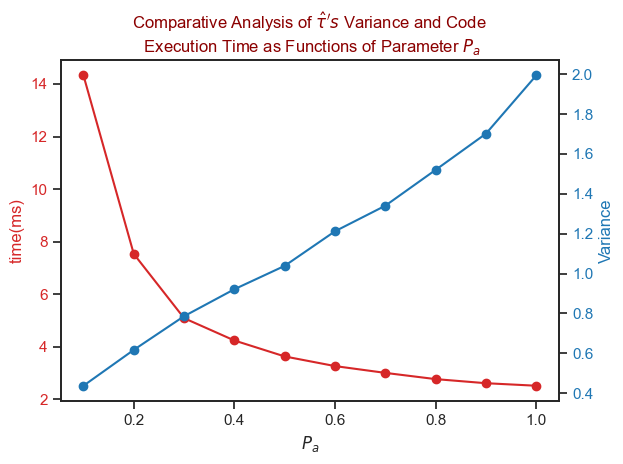
\includegraphics[width=\textwidth]{figures/重随机化Pa的影响.png} % 替换为实际的图片文件名
        \caption{不同$P_a$下$\hat{\tau}$的方差和平均重随机化时间($\tau=3.0$)}
       \label{fig:Comparative stats Analysis of Average Treatment Effects by Pa}
    \end{minipage}\hfill
    \begin{minipage}{0.3\textwidth}
        \centering
        \begin{tabular}{lcc}
            \hline
        $P_a$ & mean & variance \\
        \hline
            0.1 & 3.00 & 0.44 \\
            0.2 & 3.00 & 0.62 \\
            0.3 & 2.99 & 0.79 \\
            0.4 & 3.01 & 0.92 \\
            0.5 & 3.02 & 1.04 \\
            0.6 & 2.99 & 1.21 \\
            0.7 & 3.00 & 1.34 \\
            0.8 & 3.00 & 1.52 \\
            0.9 & 2.98 & 1.70 \\
            1.0 & 3.02 & 1.99 \\
            \hline
        \end{tabular}
        \caption{不同$P_a$下平均处理效应的估计$\hat{\tau}$的统计结果($\tau=3.0$)}
        \label{tab:Comparative stats Analysis of Average Treatment Effects by Pa}
    \end{minipage}
\end{figure}

对于不同的$P_a$,我们可以构造出不同的可接受随机化函数。在这一部分中,我们从0.1到1间隔为0.1选取了10个$P_a$,分别进行重随机化实验,得到了10组平均处理效应的估计$\hat{\tau}$。它们的均值和方差的结果如图\ref{tab:Comparative stats Analysis of Average Treatment Effects by Pa}所示。除此以外,对于不同的$P_a$,相应的平均重随机化耗时也被绘制在图\ref{fig:Comparative stats Analysis of Average Treatment Effects by Pa}中。从中我们可以发现,随着选取的$P_a$的增大,$\hat{\tau}$的方差也会逐渐增大,与此同时,平均的计算时间也会减小。在重随机化中,平均计算时间和估计的准确性不可兼得。采用重随机化时,实验设计者往往需要在平均处理效应的估计的准确性和平均计算时间中做好平衡。

\section{本章小结}
本章通过随机生成服从多元正态分布的协变量$\mathbf{X}$进而根据线性可加模型和分组结果模拟出实验结果$\mathbf{Y}$。接着本章阐述了不同随机化方法的具体实验流程和相应的参数设置。根据以上的参数设置,通过10000次模拟,得到5组$\hat{\tau}$的结果。重随机化、A/A test、区组随机化、分层随机化对$\tau$的估计都保持了无偏性,且使用重随机化和分层随机化后,$\hat{\tau}$的方差上有很大程度下降。在重随机化实验中,平均处理效应估计$\hat{\tau}$的方差随着$P_a$的增大而增大,同时平均计算时间减小。因此,实验设计者在采用重随机化时需要在估计的准确性和计算时间之间取得平衡。
